\documentclass[aspectratio=169]{beamer}

\usetheme{Madrid}
\usecolortheme{default}
\setbeamertemplate{navigation symbols}{}

\usepackage{booktabs}
\usepackage{graphicx}

\title{From ImageNet to EuroSAT}
\subtitle{Transfer Learning, When Transfer Helps, and Catastrophic Forgetting}
\author{Ruiquan Qiao \and Tiancheng Xia \and Guangde Shi}
\institute{COMP6242 Deep Learning Group Project}
\date{Semester 1, 2026}

\begin{document}

\begin{frame}
  \titlepage
\end{frame}

\begin{frame}{Video Focus}
  \begin{itemize}
    \item 5-minute project video with contributions from all group members.
    \item Explain the problem, method, and findings clearly.
    \item Use visuals to support one coherent narrative rather than every detail.
  \end{itemize}
\end{frame}

\begin{frame}{Project Goal}
  \begin{itemize}
    \item Main task: adapt an ImageNet-pretrained ResNet-18 to classify EuroSAT remote sensing scenes.
    \item Main question: does transfer learning help more than training from scratch?
    \item Supporting question 1: when does transfer help most?
    \item Supporting question 2: how much ImageNet capability is forgotten after adaptation?
  \end{itemize}
\end{frame}

\begin{frame}{Experimental Setup}
  \begin{itemize}
    \item Backbone: ResNet-18 with official ImageNet-1K pretrained weights.
    \item Main dataset: EuroSAT with 18,900 train / 4,050 val / 4,050 test images.
    \item Strategies: \texttt{scratch}, \texttt{linear\_probe}, \texttt{partial\_ft}, \texttt{full\_ft}.
    \item Shared setting: 8 epochs, batch size 32, AdamW, learning rate $3\times 10^{-4}$.
    \item Extra analyses:
    \begin{itemize}
      \item Same-size cross-domain: EuroSAT vs CIFAR-10
      \item Same-domain data-size: EuroSAT 10\%, 30\%, 60\%, 100\%
    \end{itemize}
  \end{itemize}
\end{frame}

\begin{frame}{Main Result on EuroSAT}
  \begin{columns}[T]
    \begin{column}{0.49\textwidth}
      \small
      \begin{tabular}{lrr}
        \toprule
        Strategy & Top-1 & Macro-F1 \\
        \midrule
        scratch & 93.21 & 93.04 \\
        linear\_probe & 88.54 & 88.33 \\
        partial\_ft & \textbf{97.78} & \textbf{97.71} \\
        full\_ft & 97.56 & 97.50 \\
        \bottomrule
      \end{tabular}

      \vspace{0.6em}
      \begin{itemize}
        \item Transfer helps only when the backbone is allowed to adapt.
        \item \texttt{partial\_ft} gives the best EuroSAT performance.
      \end{itemize}
    \end{column}
    \begin{column}{0.49\textwidth}
      \centering
      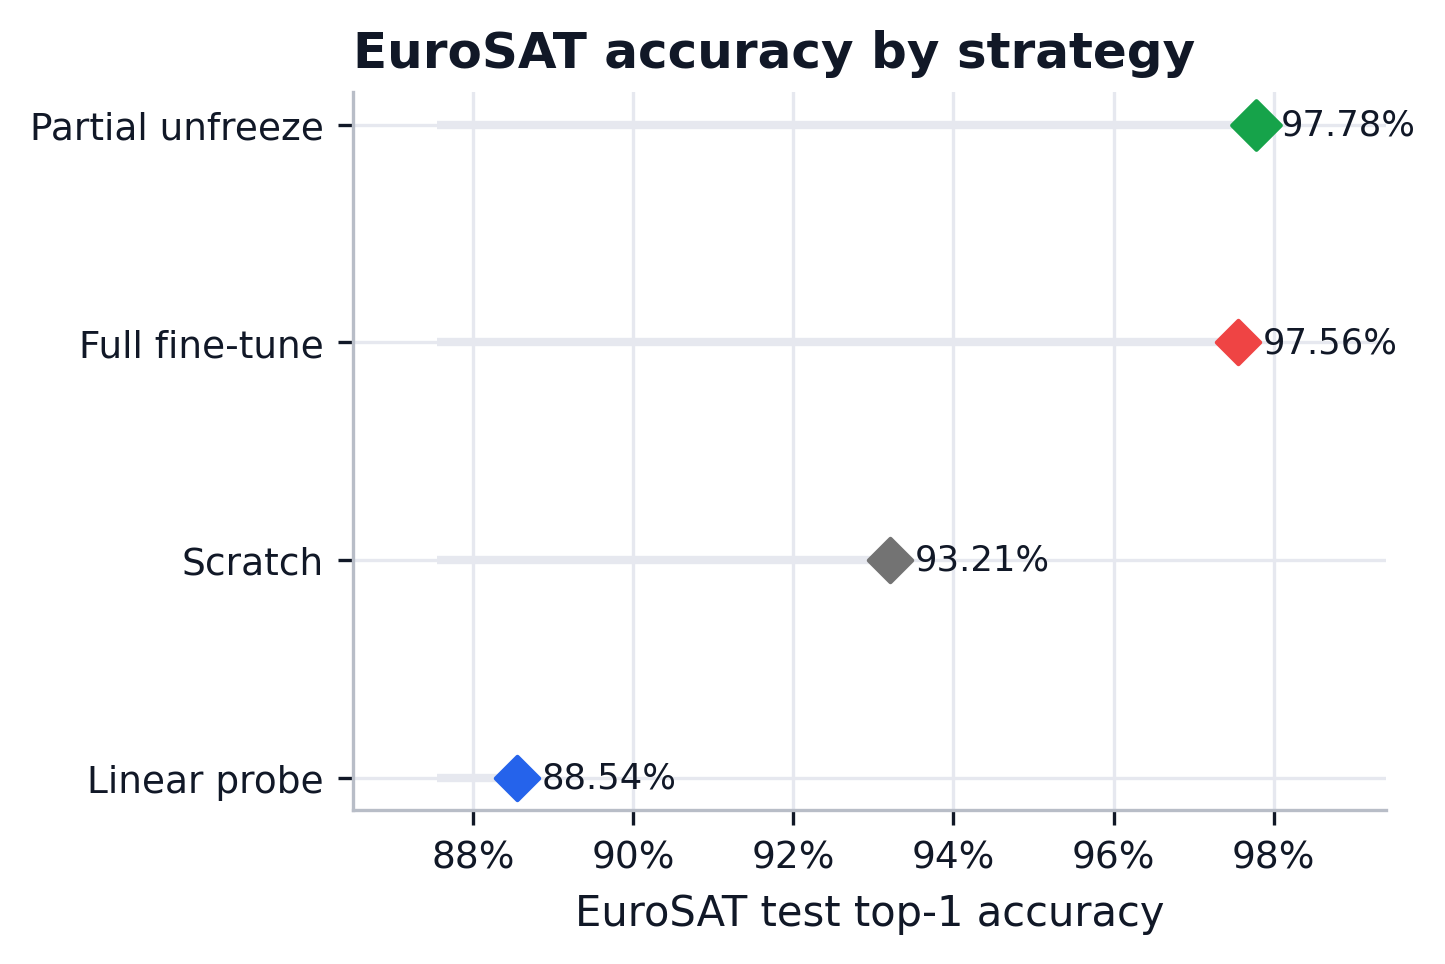
\includegraphics[width=\linewidth]{../outputs/eurosat_ablation/test_top1_acc.png}
    \end{column}
  \end{columns}
\end{frame}

\begin{frame}{Forgetting on ImageNet}
  \begin{columns}[T]
    \begin{column}{0.50\textwidth}
      \small
      \begin{tabular}{lrr}
        \toprule
        Strategy & Forgetting & EuroSAT Top-1 \\
        \midrule
        linear\_probe & 37.73 & 88.54 \\
        partial\_ft & 69.26 & \textbf{97.78} \\
        full\_ft & \textbf{69.64} & 97.56 \\
        \bottomrule
      \end{tabular}

      \vspace{0.6em}
      \begin{itemize}
        \item Linear probing preserves more ImageNet ability.
        \item Stronger EuroSAT adaptation causes much larger forgetting.
      \end{itemize}
    \end{column}
    \begin{column}{0.48\textwidth}
      \centering
      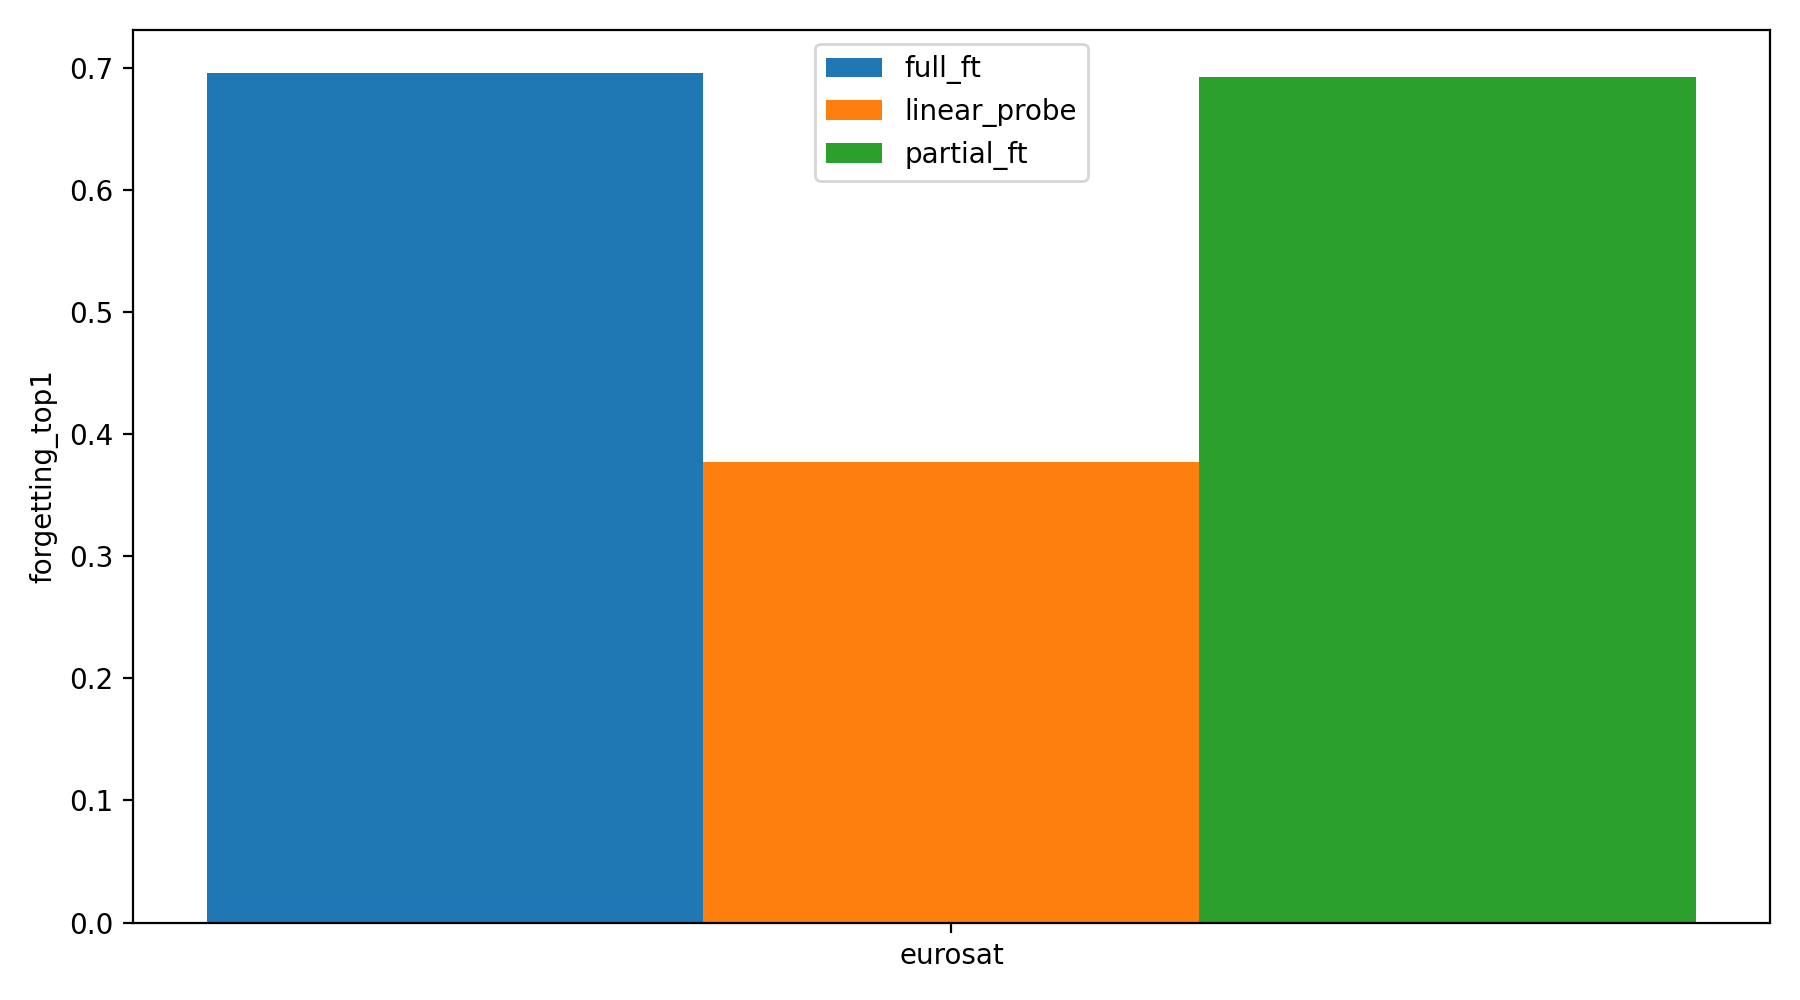
\includegraphics[width=\linewidth]{../outputs/forgetting_main/forgetting_top1.png}
    \end{column}
  \end{columns}
\end{frame}

\begin{frame}{When Transfer Helps}
  \begin{itemize}
    \item Cross-domain comparison: CIFAR-10 receives larger transfer gain than EuroSAT.
    \item Data-size comparison: transfer is most valuable in the low-data EuroSAT setting.
    \item Together, these experiments show that transfer benefit depends on target domain and label budget.
  \end{itemize}
\end{frame}

\begin{frame}{Team Contributions and Takeaways}
  \begin{itemize}
    \item Ruiquan Qiao: main experiment and corresponding forgetting analysis.
    \item Tiancheng Xia: same-size cross-domain analysis and corresponding forgetting analysis.
    \item Guangde Shi: data-size analysis and corresponding forgetting analysis.
    \item Takeaway: ImageNet transfer helps EuroSAT, but strong fine-tuning also causes severe forgetting on ImageNet.
  \end{itemize}
\end{frame}

\end{document}
